\documentclass[14pt,a4paper,report]{report}
\usepackage[a4paper, mag=1000, left=2.5cm, right=1cm, top=2cm, bottom=2cm, headsep=0.7cm, footskip=1cm]{geometry}
\usepackage[utf8]{inputenc}
\usepackage[english,russian]{babel}
\usepackage{indentfirst}
\usepackage[dvipsnames]{xcolor}
\usepackage[colorlinks]{hyperref}
\usepackage{listings} 
\usepackage{fancyhdr}
\usepackage{caption}
\usepackage{amsmath}
\usepackage{latexsym}
\usepackage{graphicx}
\usepackage{amsmath}
\usepackage{booktabs}
\usepackage{array}
\hypersetup{
	colorlinks = true,
	linkcolor  = black
}

\usepackage{titlesec}
\titleformat{\chapter}
{\Large\bfseries} % format
{}                % label
{0pt}             % sep
{\huge}           % before-code


\DeclareCaptionFont{white}{\color{white}} 

% Listing description
\usepackage{listings} 
\DeclareCaptionFormat{listing}{\colorbox{gray}{\parbox{\textwidth}{#1#2#3}}}
\captionsetup[lstlisting]{format=listing,labelfont=white,textfont=white}
\lstset{ 
	% Listing settings
	inputencoding = utf8,			
	extendedchars = \true, 
	keepspaces = true, 			  	 % Поддержка кириллицы и пробелов в комментариях
	language = C++,            	 	 % Язык программирования (для подсветки)
	basicstyle = \small\sffamily, 	 % Размер и начертание шрифта для подсветки кода
	numbers = left,               	 % Где поставить нумерацию строк (слева\справа)
	numberstyle = \tiny,          	 % Размер шрифта для номеров строк
	stepnumber = 1,               	 % Размер шага между двумя номерами строк
	numbersep = 5pt,              	 % Как далеко отстоят номера строк от подсвечиваемого кода
	backgroundcolor = \color{white}, % Цвет фона подсветки - используем \usepackage{color}
	showspaces = false,           	 % Показывать или нет пробелы специальными отступами
	showstringspaces = false,    	 % Показывать или нет пробелы в строках
	showtabs = false,           	 % Показывать или нет табуляцию в строках
	frame = single,              	 % Рисовать рамку вокруг кода
	tabsize = 2,                  	 % Размер табуляции по умолчанию равен 2 пробелам
	captionpos = t,             	 % Позиция заголовка вверху [t] или внизу [b] 
	breaklines = true,           	 % Автоматически переносить строки (да\нет)
	breakatwhitespace = false,   	 % Переносить строки только если есть пробел
	escapeinside = {\%*}{*)}      	 % Если нужно добавить комментарии в коде
}

\begin{document}

\def\contentsname{Содержание}

% Titlepage
\begin{titlepage}
	\begin{center}
		\textsc{Санкт-Петербургский Политехнический 
			Университет Петра Великого\\[5mm]
			Кафедра компьютерных систем и программных технологий}
		
		\vfill
		
		\textbf{Отчёт по лабораторной работе №2\\[3mm]
			Курс: «Администрирование компьютерных сетей»\\[3mm]
			Тема: «Тестирование компьютерной сети на основе TCP/IP»\\[35mm]
			}
	\end{center}
	
	\hfill
	\begin{minipage}{.5\textwidth}
		Выполнил студент:\\[2mm] 
		Ерниязов Тимур Ертлеуевич\\
		Группа: 13541/2\\[5mm]
		
		Проверил:\\[2mm] 
		Малышев Игорь Алексеевич
	\end{minipage}
	\vfill
	\begin{center}
		Санкт-Петербург\\ \the\year\ г.
	\end{center}
\end{titlepage}

% Contents
\tableofcontents
\clearpage
\chapter{Лабораторная работа №2}
\section{Цели работы}
\begin{enumerate}
\item Изучение утилит и систем администрирования TCP/IP-сетей.
\item Мониторинг и анализ характеристик TCP/IP-сетей.
\end{enumerate}

\section{Сведения о системе}
Работа производилась на реальной системе, со следующими характеристиками:

\begin{center}
\begin{tabular}{ c c  }
Элемент & Значение \\ 
Имя ОС & Майкрософт Windows 10 Pro (Registered Trademark)\\ 
Версия&10.0.16299 Сборка 16299\\
RAM &16 ГБ\\ 
Процессор&Intel(R) Core(TM) i5-7300HQ CPU @ 2.50GHz, 2496 МГц \\ 
\end{tabular}
\end{center}


Для выполнения работы использовалась \textbf{VMware Workstation 12 pro (12.5.7 build-5813279)}
В качестве сети для экспериментов, использовалась ККС из прошлой работы.

\section{Оценка пропускной способности}
В качестве утилиты для оценки пропускной способности была выбрана \textbf{iperf}.  Iperf — кроссплатформенная консольная клиент-серверная программа, предназначена для тестирования пропускной способности интернет канала между двумя компьютерами.

Измерение осуществляется следующим образом, на одном ПК запускаем iperf в режиме «сервер», на втором в режиме «клиент» с указанием ip-адреса первого ПК («сервера»). Через заданное время показывается измеренная информация. 

В работе использовалась \textbf{версия} 2.0.5
\subsection{Установка}
На \textbf{NetBsd}, были выполнены команды:
\begin{enumerate}
\item Загрузка iperf
\begin{enumerate}
\item Подключение к ftp серверу, к папке с пакетами для моей версии NetBSD
\begin{lstlisting}[language={}]
ftp -i ftp://ftp.netbsd.org/pub/pkgsrc/packages/NetBSD/x86_64/7.1.1/All/
\end{lstlisting}
\item Загрузка последней версии
\begin{lstlisting}[language={}]
mget iperf-2.0.5nb1.tgz
\end{lstlisting}
\item Завершение работы ftp
\begin{lstlisting}[language={}]
quit
\end{lstlisting}
\end{enumerate}
\item Создаем папку и разархивируем туда архив
\begin{lstlisting}[language={}]
mkdir iperf
tar -xzf iperf-2.0.5nb1.tgz -C /root/iperf
\end{lstlisting}
\item Утилита для запуска находится по пути \textbf{/root/iperf/bin}
\end{enumerate}

На \textbf{FreeBSD}, были выполнены команды:
\begin{lstlisting}[language={}]
cd /usr/ports/benchmarks/iperf
make install clean
\end{lstlisting}
На \textbf{Kali Linux}, была выполнена команда:
\begin{lstlisting}[language={}]
apt-get install iperf
\end{lstlisting}
На \textbf{Windows XP} были скачены бинарные файлы программы.

\subsection{Тестирование}
На хосте с FreeBSD запущен сервер iperf
\begin{lstlisting}[language={}]
iperf -s
\end{lstlisting}
На машинах(Kali Linux, NetBSD, Windows XP) iperf запущен в качестве клиента, командой:
\begin{lstlisting}[language={}]
iperf -c 192.168.40.2
\end{lstlisting}
В результате были получены следующие данные:


\begin{center}
\begin{tabular}{ c c c }
NetBSD & Kali Linux & Windows XP\\ 
1.47 Гбит/c & 1.62 Гбит/c & 5.81 Мбит/c\\ 
\end{tabular}
\end{center}

\section{Карта сети}
Для изучения сети использована программа \textbf{10-Страйк: Схема Сети}(версия 3.32), установленная на Windows XP.

При запуске программы, были указаны следующие диапазоны для сканирования:
\begin{itemize}
\item 192.168.32.1-192.168.32.254;
\item 192.168.40.1-192.168.40.254;
\item 192.168.80.1-192.168-80.254;
\item 192.168.120.1-192.168.120.254.
\end{itemize}
В качестве параметров тестирования выбрать ICMP-ping. 

После чего начнется сканирование данных диапазонов адресов. Программа построила следующую карту сети:
\begin{figure}[h]
  \centering
  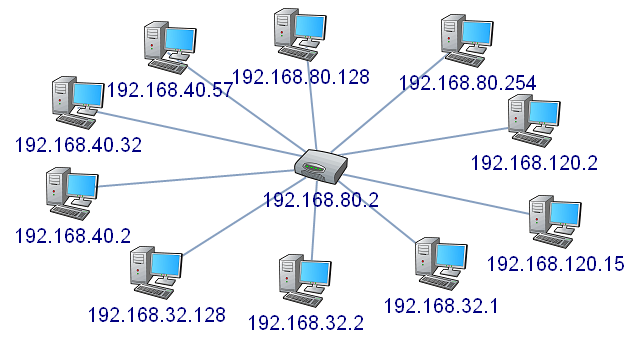
\includegraphics[width=.7\textwidth]{img/3}
  \caption{Карта сети}
\end{figure}
Программа не смогла определить точную карту сети, типы операционных систем, она видит лишь ближайший маршрутизатор, в данном случае – это FreeBSD (хост 192.168.80.2).
\section{Поиск уязвимостей}
В качестве программы по поиску уязвимостей была выбрана \textbf{X-Spider}(версия 7.7), которая была установлена на Windows XP.

Перед сканированием были добавлены следующие адреса интерфейсов:

\begin{itemize}
\item 192.168.80.128(Windwos XP);
\item 192.168.40.2(FreeBSD);
\item 192.168.80.2(FreeBSD);
\item 192.168.120.2(FreeBSD);
\item 192.168.120.15(Windows 98);
\item 192.168.40.32(Kali Linux);
\item 192.168.40.57(NetBSD);
\item 192.168.32.128(NetBSD).
\end{itemize}


По итогам работы, были выявлены следующие уязвимости:
\begin{itemize}
\item Windows XP
\begin{itemize}
\item имя операционной системе;
\item сервисом NTP открыт порт 123 по UDP;
\item сервисом RPC Windows открыт порт 135 по TCP;
\item сервисом NBNS открыт порт 137 по UDP;
\item сервисом NetBIOS открыт порт 139 по TCP.
\end{itemize}
\item Windows 98
\begin{itemize}
\item имя операционной системе;
\item сервисом NetBIOS-SSN открыт порт 137 по UDP;
\item сервисом NetBIOS открыт порт 139 по TCP.
\end{itemize}
\end{itemize}
В системах unix слабых мест не обнаружено.
\section*{Вывод}
В результате выполнения данной лабораторной работы была протестирована сеть на основе TCP/IP. 

Оценка пропускной способности показала свехвысокую скорость для ос семейства unix и весьма медленную для windows xp. Возможно это связано с кроссплатформенностью утилиты для тестирования и различных настроек операционных систем.

Утилита для построения карты сети, показала некорректную карту сети, что о говорит о сложности построения реальной карты сети.

Тестирование на уязвимости показало, что уязвимостям подвержены ОС семейства Windows, в то время как на unix системах уязвимостей найдено не было.

Для предотвращения подобных уязвимостей, необходимо использовать операционные системы актуальных версий(с последними обновлениями). Также желательно наличие какого-либо специализированного ПО для защиты системы.
%------------------------------------------------------------------------------

%\addcontentsline{toc}{section}{Список литературы}
%\bibliography{thesis}
%\bibliographystyle{ugost2008}

\end{document}